
%\documentclass[letterpaper, 10 pt, conference]{ieeeconf}  % Comment this line out
                                                          % if you need a4paper
\documentclass[a4paper, 10pt, conference]{ieeeconf}      % Use this line for a4
\usepackage[pdftex]{graphicx}
\usepackage{nameref}

%Settings for captions (Currently small text, bold and Sans Serif
\usepackage[font={small, bf, sf}]{caption}

%%% LITTERATURLISTE %%%
\usepackage[square,numbers]{natbib}
\usepackage{url}

%For ÆØÅ
\usepackage[utf8]{inputenc}
\usepackage{nameref}

%For inserting a PDF into the report
\usepackage{pdfpages}

%equations
\usepackage{amsmath}

%\begin{comment}
\usepackage{verbatim}                
                
                                                          % paper

% \IEEEoverridecommandlockouts                              % This command is only
                                                          % needed if you want to
                                                          % use the \thanks command
% \overrideIEEEmargins
% See the \addtolength command later in the file to balance the column lengths
% on the last page of the document

\title{\LARGE \bf
Drive-LaB: An Experimental Platform for Usage Based Car Insurance
}
\author{Johan Leth Gregersen, Morten Møller Jakobsen and Casper Holst Laustsen% <-this % stops a space
\thanks{*The Department of Computer S, Aalborg University}%
}


\begin{document}



\maketitle
\thispagestyle{empty}
\pagestyle{empty}


%%%%%%%%%%%%%%%%%%%%%%%%%%%%%%%%%%%%%%%%%%%%%%%%%%%%%%%%%%%%%%%%%%%%%%%%%%%%%%%%

\begin{abstract}
Usage-based insurance is currently surfacing both in research and within insurance companies. There are however a lack of actual products, with those that exist being experimental and limited to small customer segments. Insurance companies are showing a clear interest in entering the market, but UBI as a product is complex, and little research exists when it comes to fully featured products. In this paper, we describe the design, implementation and experimentation of Drive-LaB, a fully featured UBI product. Drive-LaB tracks time and location in order to determine risks associated with driving style and environment. The system is supported by a complex backend system featuring an advanced data warehouse. On the front-end however, the system offers an easy-to-use interface for location tracking. Furthermore, users are able to see detailed statistics about their trips.
\end{abstract}

%%%%%%%%%%%%%%%%%%%%%%%%%%%%%%%%%%%%%%%%%%%%%%%%%%%%%%%%%%%%%%%%%%%%%%%%%%%%%%%%
\section{INTRODUCTION}\label{sec:intro}
Usage-based car insurance (UBI) has been researched actively over the last decade. Insurance companies are showing interest in making UBI a reality, and some have even launched experimental products \citep{allstate_ubi} \citep{progressive_ubi} \citep{qbe_ubi}. Achieving a fully functional UBI product is a complex task involving difficult design choices and numerous technical challenges. Several research papers attempts to address specific concerns such as data quality \citep{art:insurtelematics} or privacy \citep{art:pripayd}. UBI products are still sparse, and to the authors knowledge no one has offered UBI as a countrywide product, anywhere in the world.
For usage-based insurance to compete with traditional car insurance, there are many potential problems and solutions, depending on the chosen design. Considering a simple UBI product, insurance companies could measure distance driven by a user, and bill for mileage accordingly. Implementing such a simple UBI system still results in several non-trivial choices. Examples could be:

\begin{itemize}
\item Whether to use dedicated devices or rely on user equipment such as smartphones
\item Which technology to rely on for accurate positioning, and at what frequency
\item How to retrieve and store data logged by individual users
\item How to let users keep track of their insurance, understand and verify that they are being billed correctly
\end{itemize}

This paper presents the entire stack of a fully functional UBI system that anyone can use. The authors attempt to move UBI away from ideas and models and one step closer to a market implementation. Having a live UBI system allows for real-life experiments, and offers unique insight into problematiques associated with different approaches to UBI. In this paper the authors try to answer the following questions:

\begin{itemize}
\item How could a complete product look like?
\item Is it possible to create a UBI system that supports a fair and understandable metrification of driving styles?
\item Are modern smartphones adequate to support UBI?

\end{itemize}

The remainder of this paper describes the process leading towards answering these questions. In Section \ref{sec:design} the system design is explained. Section \ref{sec:implementation} describes the implementation of the system. Section \ref{sec:experiments} describes experiments made possible by releasing the system into a public domain. Finally, the authors provide answers to the problem statement based on the results of the experiments, followed by a conclusion in Section \ref{sec:conclusion}.

\subsection{Prerequisites}\label{subsec:prereq}
Drive-LaB is based on the paper \textit{An Advanced Usage Based Insurance And Privacy-Secure Pricing Model}\citep{sw9_report}. The project features a metric-based scoringmodel for UBI, and focuses on being intuitive and understandable. Furthermore, it features an advanced data warehouse capable of storing all required data for supporting the described scoringmodel. Drive-LaB utilizes both the data warehouse and metric-based scoringmodel, although with certain improvements. The data warehouse implemented for Drive-LaB can be found in Appendices, Figure \ref{app:fig:newdatawarehouse}. Most notably, the \texttt{SubtTripFact} table has not been implemented in Drive-LaB. Instead, two new tables are introduced, namely \texttt{Competition Information} and \texttt{CompetingIn}.

The scoringmodel has not been altered, although its flexibility has allowed us to create a more fitting policy for the system. The policy used for experiments will be described in Section \ref{sec:experiments}. Each metric delinquency is divided into 8 different intervals, with different weights for each interval. Each metric is scored by the following algorithm:

$$
\left( \frac { \sum _{ i }^{ n }{ \left( { interval }_{ i }*\quad { weight }_{ i } \right)  }  }{ 100 }  \right) \quad -\quad 1
$$

This results in an aggregated weight. Roadtypes and Critical time period are scored linearly, calculated by multiplying the aggregated weight with the amount of delinquencies. Speeding, Accelerations, Brakes and Jerks are all evaluated polynomially. The aggregated weight is fed into a polynomial equation determined by the policy, resulting in a final aggregated weight which is multiplied with the amount of delinquencies.

\begin{align*}
ax^{y} + bx + c\quad \quad \quad \quad \quad \quad \quad \quad \quad \quad \quad \\
where\quad x = AggregatedWeight
\end{align*}

The full description of the scoringmodel is described in \citep{sw9_report} at Section 5.1.


\input{Content/Design/Design}

\section{IMPLEMENTATION}\label{sec:implementation}

In the following section the implementation of Drive-LaB is described.

The backend of Drive-LaB covers the 5 layers described in Section \ref{subsec:backend_design}. It spans over 8042 lines of code, written in C\# in Visual Studio. The frontend application is implemented as an Android application. It spans over 19192 lines of code, written in Java and XML, in Android Studio.

The system  makes use of 2 different servers. The first server, being the API server, is a single core server with a Intel(R) Xeon(R) CPU E5-2650 v3 @ 2.30GHz processing unit, and 6GB RAM. The second server is an 8-core server with an AMD Opteron(tm) Processor 6376 processing unit, and 16GB RAM.
\subsection{Frontend}\label{subsec:frontend_implementation}
A goal for Drive-LaB is to be easily accessible. To fulfill this goal, Drive-LaB is developed for Android. As of 2015 Q2, over 80\% of shipped smartphones use the Android OS\citep{smartphone_market_share}. Choosing Android as platform has allowed for the release of Drive-LaB on Google Play\citep{google_play_drivelab}, making it accessible for the vast majority of smartphone users. Furthermore, the implementation of Drive-LaB supports Android 4.0 – 6.0.1, making it compatible with over 97\% of current Android devices\citep{android_version_distribution}.
As mentioned in \ref{subsec:frontend_design}, the application has two responsibilities; data collection and data presentation. These responsibilities are mirrored in the structure of the application, seen in \ref{fig:frontend_components}. The application consists of two major components. One is the user interface, consisting of 10 different Android activities\citep{android_activity}. The interface presents data for the user, and allows for interaction with \texttt{Location Service}, the second component.\texttt{Location Service} is an Android Service\citep{android_service}. It runs separately from the rest of the application, in that it has its own process. It is however entirely controlled by the user interface as seen in Section \ref{subsubsec:service_communication}. The \texttt{Location Service} is responsible for all location logging. Running the service separately allows for a lifecycle independent of any \texttt{Activity} bound to it. In effect, the Android device can still be used normally. The application can be closed, and the screen turned off, saving battery. This will not affect the \texttt{Location Service} in any way.

\begin{figure}[tb]
\centering
\includegraphics[width=0.465\textwidth]{Pictures/frontend_components}
\caption{The frontend consists of two components, running separately from each other}
\label{fig:frontend_components}
\end{figure}

\subsubsection{Service Communication}\label{subsubsec:service_communication}
The downside of having \texttt{Location Service} running in a process separate from the rest of the application, is that communication becomes non-trivial. With the chosen setup, there is no support for synchronous communication, method invocation, or even two-way communication. The alternative method of communication is illustrated in Figure \ref{fig:application_service_communication}.   \texttt{Location Service} and \texttt{User Interface} represents a running instance of a \texttt{Service} and an arbitrary \texttt{Activity} respectively. For these components to communicate, an implementation of the interface \texttt{ServiceConnection} is required\citep{android_serviceconnection}.  The \texttt{ServiceConnection} is bound to the \texttt{Location Service} using \texttt{bindService}\citep{android_bindservice}. Upon a successful connection to the \texttt{Location Service}, the \texttt{ServiceConnection} instantiates a \texttt{Messenger}\citep{android_messenger} which is able to send messages asynchronously. Looking at the \texttt{Location Service} in figure \ref{fig:application_service_communication}, incoming messages are first caught by a \texttt{Handler}\citep{android_handler} class. By extending this class and overriding its \texttt{handleMessage} method, the \texttt{Location Service} is able to determine a course of action, depending on the message sent.

\begin{figure}[tb]
\centering
\includegraphics[width=0.465\textwidth]{Pictures/application_service_communication}
\caption{Two-way communication path between Location Service and User Interface}
\label{fig:application_service_communication}
\end{figure}

Often, the \texttt{Location Service} is required, not only to perform an action, but also respond to incoming messages. The \texttt{Location Service} is however unable to reference a calling \texttt{Activity}. Instead, the \texttt{Location Service} utilizes \texttt{sendBroadcast}\citep{android_sendbroadcast} which issues a message globally on the device. Returning to the \texttt{User Interface} side of figure \ref{fig:application_service_communication}, the receiving \texttt{Activity} can then listen for the message using a \texttt{BroadcastReceiver}\citep{android_broadcastreceiver} and act accordingly to the content of the broadcasted message. 

\subsubsection{Location Logging}\label{subsubsec:location_logging}
\texttt{Location Service} is responsible for the continuous retrieval of location updates, when demanded. Retrieving location updates through Android is done using the Google Play services location APIs, specifically the \texttt{FusedLocationProviderApi}\citep{android_fusedlocationproviderapi}. This API is able to automatically choose the best location provider, maximizing the possible precision and availability of location updates. Locations can therefore be based on both GPS, Cell-ID, and Wi-Fi. To achieve the desired quality and frequency of locations, these settings are used when requesting locations through the FusedLocationProviderApi:

\begin{itemize}
\item Desired interval: 1000ms
\item Fastest interval: 1000ms
\item Priority: High Accuracy
\end{itemize}

These settings enables Drive-Lab to receive locations exactly once every second whenever possible. Locations are furthermore pinpointed as exact as possible, regardless of battery consumption. This will usually result in GPS positions, as this is generally the more accurate option.
\subsection{Backend implementation}\label{subsec:backend_impl}
The servers are virtual machines running Ubuntu, a GNU/Linux operating system, and does not naturally run any .exe programs. Mono is an open source implementation of .NET, capable of running C\# software on Ubuntu \citep{mono}. This causes some implications when porting from initial use of Visual Studio to Mono, and these implications are stated during the implementation description below. 



\subsubsection{API Server}\label{subsec:impl_api_server}
As portrayed in Figure \ref{fig:backend_design} the API server consists of 3 layers described in this section.

The communication layer is fully implemented in C\# as a RESTful Web Service API, using the built-in .NET \texttt{ServiceModel} library. It is implemented following the design described in Section \ref{sec:api_server}. The communication layer includes thorough error-handling along with an error-reporting system. It is critical that the communication layer does not crash, because the access to the Drive-LaB backend will crash with it. The error-handling ensures that corrupted data being processed in the logic layer, does not cast exceptions back to the communication layer. Also, by using the .NET RESTful library, a series of error-handling tasks is conducted automatically. As example, if a client targets a non-existent service endpoint, or if a client use a wrong HTTP verb, the API will return a corresponding HTTP error code.

The logic layer is implemented in C\# using regular OOP-style programming. It contains many classes and methods to handle the variety of functionality handled by this layer. A majority of this functionality is to create appropriate C\# objects, either based on JSON data received from the communication layer, or data received in \texttt{DataRow} format from the DAL. DataRow is a .NET specific data type, designed to hold a row of data received from a database, which is what the DAL returns to the logic layer.  

The logic layer uses Json.NET, a popular JSON framework for .NET \citep{json_dot_net}. Using a third party framework to support JSON serialization and deserialization is neccessary, because Mono does not contain Visual Studio libraries to support this task. Another library that is not implemented in Mono is \texttt{Device.Location}, which offers the type \texttt{GeoCoordinate} in C\#. It is used to store spatio-temporal data, and offers functionality like computing distance between two coordinates. A third party library called GeoCoordinatePortable offers this functionality while also being Mono-compatible \citep{geocoordinateportable}. Therefore, this library is used as substitute.

Last is the DAL. This layer is implemented using a combination of SQL and C\#. It makes use of \texttt{Npgsql} \citep{npgsql}, a .NET data provider for PostgreSQL, which makes it very easy to write SQL statements and C\# code in the same IDE. 
\subsubsection{Storage Server}\label{subsec:impl_storage_server}
In the implemented system, it was found to be simpler to implement the trip-processing layer as part of the logic layer. This does opposes the design decision to optimize the computational resources offered by the more powerful server. Monitoring the ongoing load on the API server, however shows that computation power is sufficient with a small set of users. The solution will however not scale well, and with more users this will have to be reworked to maximize the performance of the system. 

The trip-processing layer contains two extensive computational schemes named \texttt{GPSFactUpdater} and \texttt{TripFactUpdater}. The former computes all measures and flags between every GPS coordinate logged during the trip. This is the foundation for the entries inserted in the \texttt{TripFact} table and therefore has to be accurate. The modular design of classes is valuable in the context of processing trips, because appropriate objects can be chosen and forwarded to the \texttt{MeasureCalculator}. The \texttt{MeasureCalculator} contains mathematical formulas for calculating measures, for example how to compute speed. Only the appropriate sub classes are sent as parameters, and the complete object is not thrown around between formulas. 

\texttt{TripFactUpdater} computes the required attributes in the \texttt{TripFact}, which is statistical groupings of the information stored in the \texttt{GPSFact} table. It uses these statistical attributes to analyze driver performance, compute optimal- and actual tripscores. The scoringmodel, used to compute the actual tripscore, can be seen in Section \ref{subsec:prereq}.

\section{EXPERIMENTS}\label{sec:experiments}

Experiments intro her

\subsection{Data Collection}\label{sec:datacollection}
Releasing Drive-LaB publically has allowed for the collection of a sizeable dataset. For this report, 51 people participated, contributing a total of 581 trips spanning 13.075 kilometers. The trips are all logged between May 1st, 2016 and June 11th, 2016. All installations of Drive-LaB uses the same setup for logging locations, ensuring a uniform premise across all contributed trips. As mentioned in Section \ref{subsubsec:location_logging}, the requested sample rate is set at 1Hz, but conditions such as hardware limitations and poor signal can block this from being possible. As such, the collected data varies in sample rate. The total average of the dataset is 0.63Hz, still making it high-frequency, but lower than the desired 1Hz.

\subsubsection{Data}\label{subsec:data}
Trips logged through Android devices contain a set of latitudes, longitudes and timestamps with 1Hz granularity. Drive-LaB does not store data permanently and therefore only holds this data in memory. Namely it uses the Android \texttt{Location} class as seen in Section \ref{android_location}. As trips are sent to the storage server, all data is treated by the intermediate server, described in Section \ref{subsec:api}. Upon reaching the storage server, all data matches the data warehouse described in \ref{sw9_report}. 

\subsubsection{Policy}\label{subsec:policy}
The trips have been evaluated based on a policy throughout the test. The policy is described in Tables \ref{tab:roadtypevalues}, \ref{tab:crittimevalues}, \ref{tab:speedingvalues}, \ref{tab:accelerationvalues} and \ref{tab:jerkbrakenvalues}. The base values for the delinquencies are described in Table \ref{tab:basevalues}. The most notable change is the polynomial scoring have been omitted, as it is uncertain how the equation directly affects the scoring of the system. It should be revised when more information about the effect is present.

\begin{table}
    \centering
    \begin{tabular}{|ll|}
    \hline
    \rowcolor{tablegreen}
    \textbf{Roadtype} & \textbf{Weight} \\ \hline
    Motorway          & 0.8               \\
    Trunk             & 0.9               \\
    Primary           & 0.95               \\
    Secondary         & 1.05            \\
    Tertiary          & 1.1             \\
    Unclassified      & 1.1             \\
    Residential       & 1.2             \\
    Service           & 1.2             \\ \hline
    \end{tabular}
    \caption{Roadtypes with weights}
    \label{tab:roadtypevalues}
\end{table}

\begin{table}
    \centering
    \begin{tabular}{|llll|}
    \hline
    \rowcolor{tablegreen}
    \textbf{Active days} & \textbf{Start} & \textbf{End} & \textbf{Weight} \\ \hline
    Monday - Friday      & 07:00:00       & 09:00:00     & 1.16             \\
    Monday - Friday      & 15:00:00       & 17:00:00     & 1.12            \\
    Saturday - Sunday    & 09:00:00       & 13:00:00     & 1.02           \\
    Saturday - Sunday    & 20:00:00       & 23:59:59     & 1.12            \\
    Saturday - Sunday    & 00:00:00       & 00:04:00     & 1.325             \\\hline
    \end{tabular}
    \caption{Critical time intervals with weights}
    \label{tab:crittimevalues}
\end{table}

\begin{table}
    \centering
    \begin{tabular}{|ll|}
    \hline
    \rowcolor{tablegreen}
    \textbf{Interval (\%)}   & \textbf{Weight} \\ \hline
    {[}0, 10{[}        & 1.3                   \\
    {[}10, 20{[}       & 1.4                   \\
    {[}20, 30{[}       & 1.5                   \\
    {[}30, 40{[}       & 1.6                   \\
    {[}40, 50{[}       & 1.7                   \\
    {[}50, 60{[}       & 1.8                   \\
    {[}60, 70{[}       & 1.9                   \\
    {[}70, $\infty${]} & 2.0                   \\ \hline
    \end{tabular}
    \caption{Speeding intervals with weights}
    \label{tab:speedingvalues}
\end{table}

\begin{table}
    \centering
    \begin{tabular}{|ll|}
    \hline
    \rowcolor{tablegreen}
    \textbf{Interval (m/s)} & \textbf{Weight} \\ \hline
    {[}6, 7{[}              & 1.05             \\
    {[}7, 8{[}              & 1.10             \\
    {[}8, 9{[}              & 1.175             \\
    {[}9, 10{[}             & 1.275             \\
    {[}10, 11{[}            & 1.40            \\
    {[}11, 12{[}            & 1.55             \\
    {[}12, 13{[}            & 1.725             \\
    {[}13, $\infty${]}      & 2.0             \\ \hline
    \end{tabular}
    \caption{Acceleration with weights}
    \label{tab:accelerationvalues}
\end{table}

\begin{table}
    \centering
    \begin{tabular}{|ll|}
    \hline
    \rowcolor{tablegreen}
    \textbf{Interval (m/s)} & \textbf{Brake Weight} \\ \hline
    {[}8, 9{[}              & 1.05 			             \\
    {[}9, 10{[}             & 1.10			              \\
    {[}10, 11{[}            & 1.175   		           \\
    {[}11, 12{[}            & 1.275  		            \\
    {[}12, 13{[}            & 1.40   		          \\
    {[}13, 14{[}            & 1.55    		          \\
    {[}14, 15{[}            & 1.725  		            \\
    {[}15, $\infty${]}      & 2.0    	   	       \\ \hline
    \end{tabular}
    \caption{Jerks and brakes with weights}
    \label{tab:jerkbrakenvalues}
\end{table}

\begin{table}
    \centering
    \begin{tabular}{|ll|}
    \hline
    \rowcolor{tablegreen}
    \textbf{Action} & \textbf{Base weight} \\ \hline
    Acceleration    & 40                   \\
    Brake           & 65                   \\
    Jerk            & 15                 \\ \hline
    \end{tabular}
    \caption{Base weights for accelerations, brakes and jerks}
    \label{tab:basevalues}
\end{table}

%
%\begin{table}
%    \centering
%    \begin{tabular}{ll}
%    \textbf{Parameter} & \textbf{Weight} \\ \hline
%    A                  & 1            \\
%    B                  & 1            \\
%    C                  & 0               \\
%    Polynomial degree  & 1            \\ \hline
%    \end{tabular}
%    \caption{Weights for all polynomial functions}
%    \label{tab:polyvalues}
%\end{table}
\subsection{System Experiments}\label{subsec:expsystem}
An important aspect of the experiments, is to validate if there is an impact on tripscores caused by the diversity of users' smartphones. In a usage-based insurance context, users needs to be treated equally, which relies entirely upon their smartphone and the GPS antenna. Two smartphones logging the same trip, should report the same tripscore. Such an analysis can be quite extensive, involving an entire market of smartphones and different versions of GPS antennas. Instead, a small initial test with a selection of different smartphones will tell whether this system is vulnerable to GPS inaccuracy. 

This small initial test will be referred to as an applicability test. An applicability test will confirm whether or not smartphones are good enough to equally score trips. It was conducted by bringing five different smartphones and two high quality GPS trackers\citep{quality_gps_device} into the same car, and recording the trip with all entities at the same time. If the system is applicable for usage-based insurance, the smartphones needs to report the same tripscores, and the route needs to be highly similar to those recorded by the high quality GPS trackers.
 
\begin{figure}[tb]
\centering
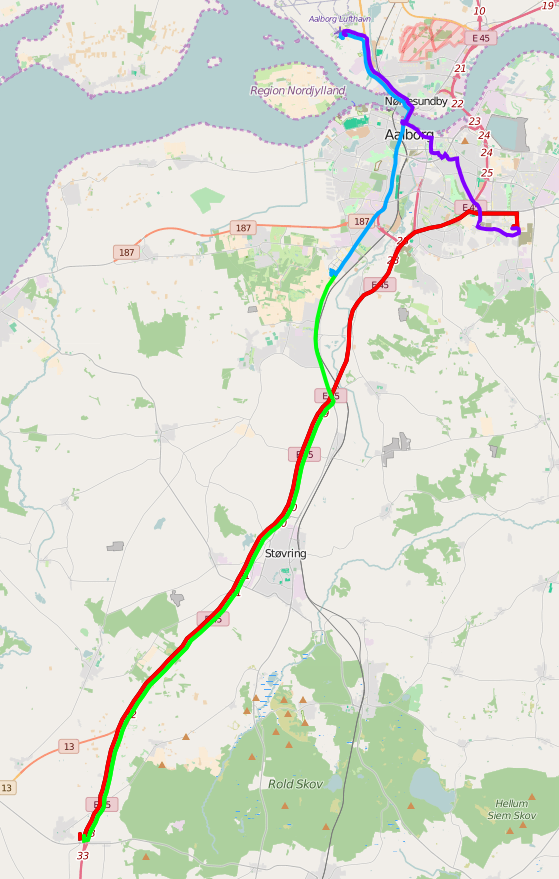
\includegraphics[width=0.465\textwidth]{Pictures/experiment_routes}
\caption{Routes traveled in the area of Aalborg during the experiment}
\label{fig:experiment_routes}
\end{figure}

With these seven devices, four trips were completed driving around in northern Jutland, in the vicinity of Aalborg. Raw data from the trips can be seen in Tables \ref{exp1trip1}, \ref{exp1trip2}, \ref{exp1trip3} and \ref{exp1trip4} in Appendices. A summary of the tripscores for each phone, during the four trips, can be seen in Table \ref{tab:smartphone_test_one}.

\begin{table*}[tb]
\centering
\caption{The tripscores from all seven recording devices, on all four trips used, during the first test}
\label{tab:smartphone_test_one}
\begin{tabular}{|l|llll|}
\hline
\rowcolor{tablegreen}

                   & \textbf{Trip 1}    & \textbf{Trip 2}    & \textbf{Trip 3}    & \textbf{Trip 4}  \\\hline
OnePlus One        & 50.191   & \ \  58.922   & 42.751   & 23.228 \\
Samsung Galaxy S5  & 40.092   & \ \ 56.781   & 24.026   & 27.530 \\
HTC One Mini 2     & 75.063   & \ \ 28.734   & 21.012   & 19.203 \\
Huawei Y330        & 81.819   &  128.056   & 50.622   & 13.082 \\
Samsung Galaxy S4  & 37.010   & \ \ 27.762   & 16.927   & 18.825 \\
BT-Q1300ST (\#1)   & 37.910   & \ \ 25.373   & 20.981   & 23.917 \\
BT-Q1300ST (\#2)   & 69.956   & \ \ 72.785   & 85.139   & 27.074 \\\hline

\end{tabular}
\end{table*}

When examining trip 1 from Table \ref{tab:smartphone_test_one} which has a length of approximately 36.200 meters, two smartphones and one high quality GPS gets a score ranging from 37.000-40.000 which is good. But the remaining four tripscores disagree with varying severity. The worst is the Huawei Y330, which score this trip 81.819. However, the Huawei Y330 only logs 23\% of the average GPS coordinates compared to the other devices. The Huawei continues this trend throughout the test, and seems unfit for use in usage-based insurance. Another alarming result in trip 1 is the degree to which the two high quality GPS devices disagrees. One scores the trip 37.910 and the other 69.956 which is a big difference.

Looking at trip 2 in Table \ref{tab:smartphone_test_one} which has a length of approximately 28.200 meters, three devices range from 25000-28750 in tripscore. The noteworthy result compared to trip 1 is, that the three devices with a low tripscore are not the same as those in trip 1.

The same pattern reoccur with trip 3 from Table \ref{tab:smartphone_test_one}, which has a length of approximately 13.400, but this time four devices gets a score ranging from 16.500-24.050, which are rather similar. The last three devices got a much higher tripscore, the highest being 85.139, approximately 535\% above the trip-length, and it was logged by one of the high quality GPS devices. To highlight the disagreement between the two high quality GPS devices, the other device got a score of 20.981. 

The pattern is broken with trip 4 from Table \ref{tab:smartphone_test_one}, where all devices range between 13.000-27.550. This may still be somewhat diversified scores, but to compare it to trip 3, the highest device only scored approximately 91\% above the trip-length from this trip, compared to 535\% in trip 3. The two high quality GPS devices also fairly agrees on the tripscore for trip 4, 23.917 and 27.075 respectively. 

When analyzing the results from this test, the immediate thought may be to throw away the smartphone as usage-based insurance component. Concern about accuracy, integrity, availability and continuity of service in standalone GPS receivers is also raised in \citep{art:challenges_smartphone_ubi} \citep{art:survey_mobile_phone_sensing} \citep{art:smartphones_for_monitoring_and_ubi} \citep{art:insurtelematics} \citep{art:in-car_positioning_technologies}. But two other factors may have influenced the results in Table \ref{tab:smartphone_test_one}. The first factor is GPS interference, in which case the test setup could have changed the results, because all the GPS devices was kept close together in a fabric container and placed in the front of the car near the windshield. This could affect the GPS receivers by interfering with each other \citep{art:gps_interference_two} \citep{art:gps_interference_one}. This position was decided upon, because a common reference point was valued in the applicability test. One article provides concrete results in terms of coverage from smartphone GPS receivers, and during an 1 hour and 15 minutes trip, 6 heavy brakes was detected with an OBD device inside the car. A total of seven smartphones was brought on this trip, and they had a coverage in the interval of 60\% to 99.7\% when detecting these brakes \citep{art:insurtelematics}, which states they are indeed vulnerable to inaccuracy. Coverage means the degree to which the smartphones align with the control-unit, in this case the OBD. The test also included outliers, false positives, and indeterminable which causes the percentages to be skewed.

The second factor is the use of third party software for map-matching of the spatio-temporal trajectories collected by the smartphones, called TrackMatching \citep{trackmatch}. TrackMatch attempts to map-match a series of spatio-temporal points to the OSM road network, and output the entire route by segments and map-adjusted GPS points. How TrackMatch decides to readjust these GPS points are uncontrollable for this system, and no module was implemented to oversee this readjusting, so this influence cannot be changed.

It was decided to repeat the applicability test and eliminate the GPS interference as much as possible. The GPS devices was arranged in the car with as much distance as possible between them. The possible margin of error by using a separated reference point was disregarded. The Huawei Y330 was also omitted. 

\begin{table*}[tb]
\centering
\caption{The tripscores from all six recording devices, on all four trips used, during the second test}
\label{tab:smartphone_test_two}
\begin{tabular}{|l|llll|}
\hline
\rowcolor{tablegreen}

                   & \textbf{Trip 1}    & \textbf{Trip 2}    & \textbf{Trip 3}    & \textbf{Trip 4}  \\\hline
OnePlus One        & 64.511  & 31.075  & 17.103  & 18.223 \\
Samsung Galaxy S5  & 46.668  & 48.169  & 19.010  & 22.779 \\
HTC One Mini 2     & 54.564  & 39.439  & 27.674  & 29.767 \\
Samsung Galaxy S4  & 37.475  & 29.242  & 16.672  & 18.094 \\
BT-Q1300ST (\#1)   & 37.800  & 30.397  & 26.440  & 25.064 \\
BT-Q1300ST (\#2)   & 41.260  & 37.029  & 36.531  & 45.327 \\\hline

\end{tabular}
\end{table*}

The test results shown in Table \ref{tab:smartphone_test_two} once again shows a considerable difference when comparing the two high quality GPS devices. But the difference is decreased substantially compared to the first test, which signifies that some external influence may have been affecting the devices. Looking at the raw data in Tables \ref{exp1trip1} through \ref{exp2trip2}, an observation is that their behavior is consistent. When looking at the amount of accelerations, brakes and jerks, one device consistently counts more than the other. BT-\#1 counted a total of 1529 of these events, whereas BT-\#2 counted a total of 3894. That is 191.13 events per trip on average for BT-\#1, and 486.75 events per trip on average for BT-\#2. This generalization of more events registered by BT-\#2 are present in both tests. This signifies that it may not be able to conclude any comparison between these two devices, because they deliver such different results.

The results from Samsung Galaxy S4, Samsung Galaxy S5 and BT-\#1 from the second test, actually compares well to the results they provided in the first test. There is an influence in the driving style, but both tests was performed by the same driver. The driver attempted to follow his personal driving style during both tests. Additionally, traffic may also influence the results in the tests, but the tests was performed in a similar time-period, both on a weekday. 

The remaining devices disagrees with their results from the first test to the second test, for atleast some of the trips. When looking at the overall result from both tests, the system is not currently applicable for usage-based insurance. This is due to the diversity in tripscores for similar trips, making it unfair to the policyholders. However, several articles raised concern about the GPS receivers, but some also suggested a way of supporting the raw data with model-based signal processing and an outlier rejection scheme \citep{art:challenges_smartphone_ubi} \citep{art:smartphones_for_monitoring_and_ubi} \citep{art:insurtelematics}. This would make the trajectories more stringent, and possibly eliminate falsely positive delinquencies caused by a jumpy GPS coordinate. It is considered a good next step to design and implement such a scheme in the system. This scheme could make each GPS receiver agree more with itself. If it could be achieved that every GPS device produces reproducible results, a calibration mechanism could eliminate the diversity caused by different GPS devices. This would ultimately cleanse the instability about accuracy, integrity, availability and continuity of service from standalone GPS receivers, and make the system robust enough to apply entirely to usage-based insurance.

\subsection{Pearson Correlation}\label{subsec:pearsoncorrelation}

In order to test the validity of our metrics and the chosen policy, a the pearson correlation between the metrics have been conducted. The point of the test is to make sure no metrics are directly correlating, meaning one of the metrics is negligible. There is a number of different reasons as to why the outcome will look as it does, and it will be discussed thoroughly. The Pearson-Correlation have been calculated on the individual scores given to a trip per each of metrics. 

The matrix of pearson correlations between the metrics is shown at table \ref{tab:pearsonmatrix}. The most notable result is the multicollinearity between accelerations and brakes, which seems rather odd as they are diametrical opposites and can per definition not exist at the same time. Another highly correlating metric is jerks having a correlation of 0.828 with both brakes and accelerations. 

\begin{table*}[tb]
\centering
\caption{This is the pearson correlation matrix between the metrics}
\label{tab:pearsonmatrix}
\begin{tabular}{l|llllll}
                      & Roadtypes & Critical Time Periods & Speeding & Accelerations & Brakes & Jerks  \\ \hline
Roadtypes             & 1         & -0.250                & -0,546   & -0.341        & -0,348 & -0,241 \\
Critical Time Periods & -0.250    & 1                     & 0.156    & 0.460         & 0.428  & 0.313  \\
Speeding              & -0,546    & 0.156                 & 1        & 0.196         & 0.195  & 0.144  \\
Accelerations         & -0.341    & 0.460                 & 0.196    & 1             & 0.971  & 0.828  \\
Brakes                & -0,348    & 0.428                 & 0.195    & 0.971         & 1      & 0.828  \\
Jerks                 & -0,241    & 0.313                 & 0.144    & 0.828         & 0.828  & 1     
\end{tabular}
\end{table*}

Looking closer at the multicollinearity between accelerations and brakes, there is a couple of different factors which affect the result. As mentioned accelerating and braking are diametrically opposite, but they are both dependant of the speed of the vehicle (as they are calculated through the change in speed). If the driver performs a big acceleration, his speed is high and he at some point needs to brake in order to decline in speed. 

\begin{figure}[tb]
\centering
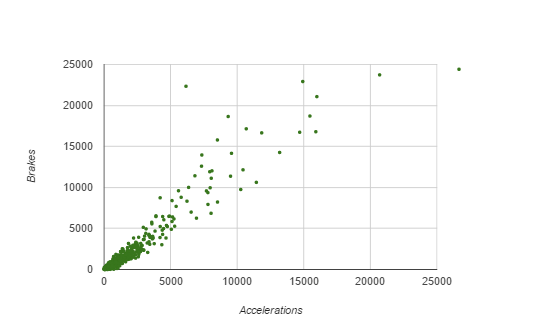
\includegraphics[width=0.465\textwidth]{Pictures/abcorrel}
\caption{The correlation between accelerations and brakes}
\label{fig:abcorrel}
\end{figure}

The figure shown at \ref{fig:abcorrel} clearly illustrates the correlation. Another reasoning as to why these metrics correlate can be the thresholds in the policy used to calculate the scores. As earlier mentioned the threshold for brakes are 8 $m/s^2$ whereas accelerations are counted from 5 $m/s^2$. If we had no thresholds and the delinquencies were scored the same, the correlation would be 1.0 as it only depended on the speed of the vehicle. 
Jerks was the metric met with the highest level of scepticism when implemented, and the correlation shows that it was not completely unwarranted. It does show a lot of correlation with both brakes and accelerations. The figure \ref{fig:ajcorrel} shows the correlation between accelerations and jerks. Jerks are as mentioned calculated as $m/s^3$, and a driver with many accelerations are almost bound to have a lot of jerks as it is hard to keep a constant acceleration.

\begin{figure}[tb]
\centering
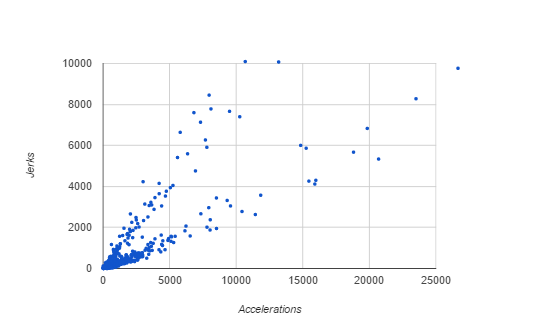
\includegraphics[width=0.465\textwidth]{Pictures/ajcorrel}
\caption{The correlation between accelerations and jerks}
\label{fig:ajcorrel}
\end{figure}


the similar correlation between the two can be answered by the correlation between accelerations and brakes. 


\subsection{Driver Profiling}\label{subsec:userprofiling}

Creating driver profiles is one of the strengths in Drive-LaB. With a descriptive set of metrics it is possible to differentiate between drivers, and create fairly accurate driver profiles without compromising the users privacy. The entire concept of a driver profile is relevant for this project due to the direct connection to the insurance industry. Naturally, it is possible to evaluate the drivers insurance costs more precisely, if the given driver profile is accurate. However driver profiles is demanded to be accurate and portray the full picture when you are dealing with paying customers\citep{art:insurtelematics} -as they need an incentive to use the product. In the remainder of this section, two random driver profiles will be reviewed and used to illustrate the capabilities in Drive-LaB to differentiate between styles of driving.  

\paragraph{Score Percentages} are a great way to differentiate between drivers. The two drivers will be referenced to as Driver 1 with an average tripscore percentage of 65,08\%, and Driver 2 with an average tripscore percentage of 39,07\%.

Beside the obvious difference in percentages, looking at where the drivers generate their scores show clear differences. Figure \ref{fig:avgmetricper} and Figure \ref{fig:piecharts} shows a comparison between the two drivers, portrayed as a bar chart and a pie chart with the distribution of the tripscore based on metrics. Looking at Driver 1, a lot of the score actually comes from accelerations at roughly 21\%, brakes at roughly 28\% and to some extend jerks at roughly 11\%. It is also worth mentioning that roadtypes actually scored negative on average. Looking at the pie chart in Figure \ref{fig:piecharts}, brakes is easily recognizable as the biggest contributor to a higher score.

\begin{figure*}[tb]
\centering
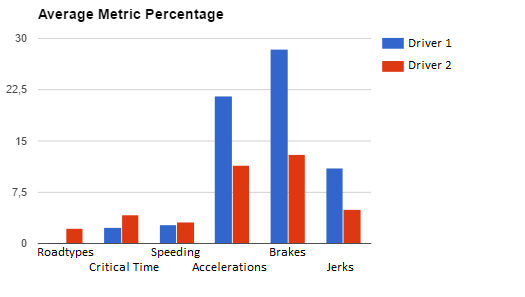
\includegraphics[width=0.465\textwidth]{Pictures/AverageMetricsPercentage}
\caption{A bar chart of the distribution of tripscore percentage by metrics for Driver 1 and Driver 2}
\label{fig:avgmetricper}
\end{figure*}

\begin{figure*}[tb]
\centering
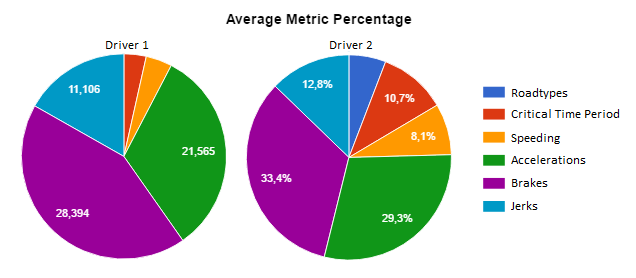
\includegraphics[width=0.95\textwidth]{Pictures/piecharts}
\caption{A bar chart of the distribution of tripscore percentage by metrics for Driver 1 and Driver 2}
\label{fig:piecharts}
\end{figure*}

Driver 2 has quite a different distribution than Driver 1, aside from a lower tripscore percentage in general. Accelerations and brakes clearly heavily influence the score in the system, however this driver have a significantly lower percentage in both of the metrics in the tripscore. This is noticeable in the pie chart in Figure \ref{fig:piecharts} which shows far less disparity between the metrics than the previous driver. 

\paragraph{Normalized Metrics} are the average metrics on a certain distance driven. For easy comparison the distance chosen is 1.000 meters. Looking at Driver 1, in Figure \ref{fig:avgmetricnorm}, Driver 1 has 6.84 points with jerks flagged given the chosen distance. Looking at Driver 2 and comparing it to Driver 1, Driver 2 nearly has half the amount of accelerations, brakes and jerks per 1.000 meters. The only metric Driver 2 has more of, given the chosen distance, is speeding.

\begin{figure}[tb]
\centering
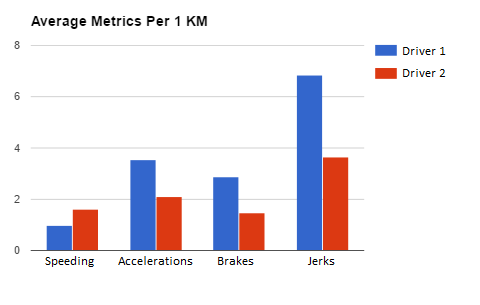
\includegraphics[width=0.465\textwidth]{Pictures/AverageMetricsNorm}
\caption{A bar chart of the metrics per 1.000 meters for Driver 1}
\label{fig:avgmetricnorm}
\end{figure}

\paragraph{Severity of Delinquencies} is one of the big tells when differentiating between drivers. It is noticeable when looking at Figure \ref{fig:car8intervals}, which represents Driver 1, there is a slight decline with a spike in the last interval. There might be several reasons as to why the last interval spike but the primary reason is that the interval is everything above a threshold, thus a much larger interval than the previous. Comparing Driver 1 to Driver 2, shown in Figure \ref{fig:car21intervals}, there is quite a different distribution.

\begin{figure*}[tb]
\centering
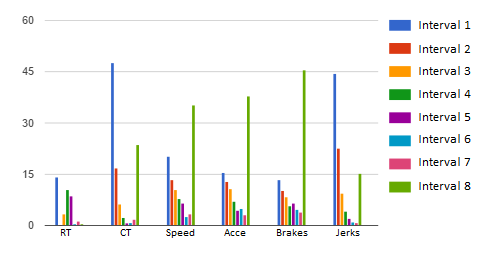
\includegraphics[width=0.95\textwidth]{Pictures/car8intervals}
\caption{A bar chart of the distribution of metrics within the intervals for Driver 1}
\label{fig:car8intervals}
\end{figure*}

\begin{figure*}[tb]
\centering
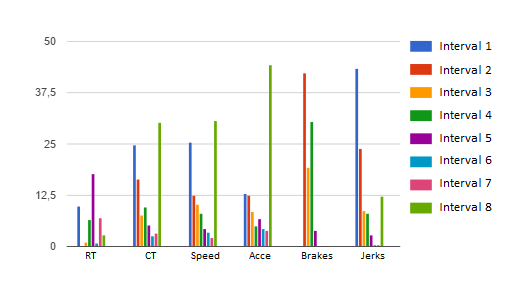
\includegraphics[width=0.95\textwidth]{Pictures/car21intervals}
\caption{A bar chart of the distribution of metrics within the intervals for Driver 2}
\label{fig:car21intervals}
\end{figure*}

It is possible to distinguish between drivers, and even more important, it is possible to create driver profiles. Given a arbitrary trip it would be possible to draw similarities between the trip and the driver profiles. From an usage-based insurance point of view, it would be possible to access the risk of a given driver. As an example, a driver with a higher amount of braking delinquencies, all represented as brakes with a hard degree, might have a higher risk of crashing and get a more expensive insurance claim.
\subsection{User Experiments}\label{subsec:userexp}

The entire system have been tested through an end user experiment involving a subset of the users. The experiment includes 10 drivers, who have been instructed to use the system for all their vehicular trips. The experiment ran from the 1st of May till the 3rd of June. As a motivator for using the system thoroughly, the user with the lowest average score percentage would win a prize at the end of the experiment. Throughout the experiments the 10 users have driven 345 trips spanning 8.190,6 kilometers.

There is several points of this experiment, and one of them is to test the system in its entirety, in a setting true to the environment the system were to eventually be release in. Therefore the setup is as true to that as possible. The frontend application was deployed on Google Play, where the test subjects downloaded and started to use the product. Throughout the experiments they were presented with a leaderboard with average scores for each of all the drivers. 
Furthermore getting user inputs on the system, whether it is easy to use or there are some obvious improvements to make. However the user feedback are still on its way.

One of the more interesting things to investigate through this experiment, is to whether or not there is any improvement in score percentages for each driver. Figure \ref{fig:tendencylines} shows the tendency lines for each of the driver throughout the test period. It is important to notice this is merely tendency lines and not projection lines. The figure shows a downward trend with 8 of the 10 drivers, with  slope ratios between -0,284 and 3,273. It shows an upward trend with the last 2 driver, with slope ratios at 0,13 and 3,54. The highest numerical slope ratios are representing the drivers with the fewest amount of trips, and drivers with 0 trips later in the test period. What this tells us is that users of the system scores slightly better when having used the system for a period of time. This either means that users of the system drives better and better depending on whether the system is indicative of a good driver.

\begin{figure*}[tb]
\centering
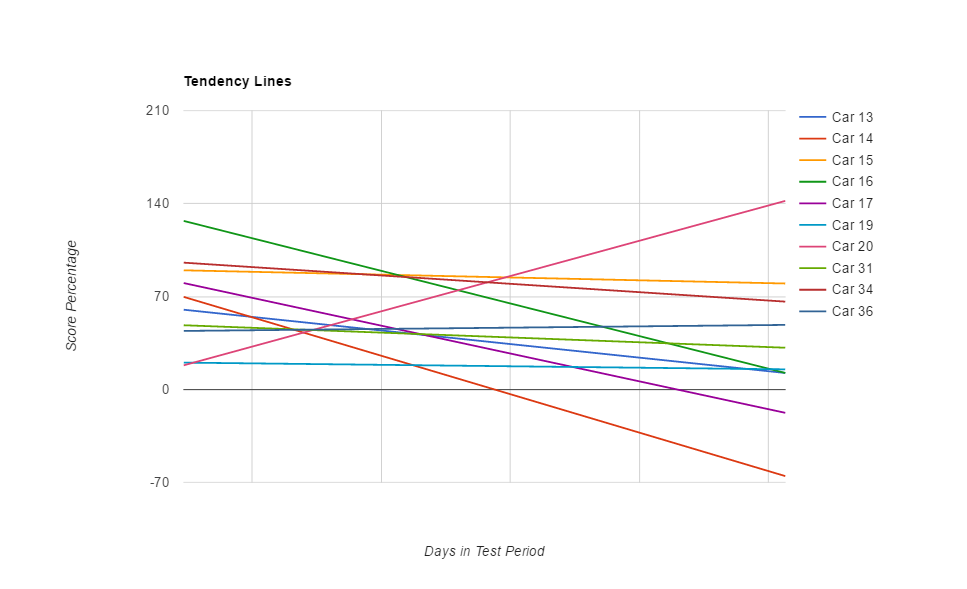
\includegraphics[width=0.95\textwidth]{Pictures/tendenslinjer}
\caption{A line chart showing the tendency lines for each individual driver}
\label{fig:tendencylines}
\end{figure*}

Lastly there it is a point to whether or not there is an incentive to keep using the system. As mentioned the winner of the experiment were to receive a prize at the end of the experiment. As shown in Figure \ref{fig:summationoftripscore} theres a slight negative tendency is score summation, but it roughly correlates with the negative slope ratios of the tendencies in trip percentages. This means there was incentive enough to keep using the system, with the given prize. In a eventual insurance environment the incentive would be a cheaper insurance for the end user -therefore given the monetary value roughly equals the prize of the experiment, there should be incentive enough.

\begin{figure*}[tb]
\centering
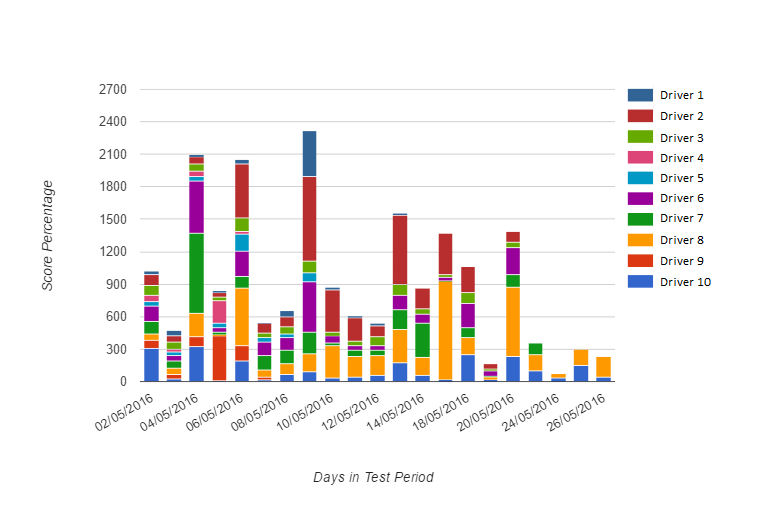
\includegraphics[width=0.95\textwidth]{Pictures/summationoftripscore}
\caption{A summation of scores based on days}
\label{fig:summationoftripscore}
\end{figure*}
 


\input{Content/RelatedWork/relatedWork}

\input{Content/Conclusion/Conclusion}

%%%%%%%%%%%%%%%%%%%%%%%%%%%%%%%%%%%%%%%%%%%%%%%%%%%%%%%%%%%%%%%%%%%%%%%%%%%%%%%%

\section*{ACKNOWLEDGMENT}

The authors thanks Kristian Torp for his supervision and valuable input to the work behind this paper.

%%%%%%%%%%%%%%%%%%%%%%%%%%%%%%%%%%%%%%%%%%%%%%%%%%%%%%%%%%%%%%%%%%%%%%%%%%%%%%%%

\bibliographystyle{chicago}
\bibliography{Litterature/litteratur}

\section*{APPENDIX}

Appendixes should appear before the acknowledgment.

\subsection*{Raw Test Data - First test}\label{app:rawtestdata1}
Raw test data one
\begin{table*}[tb]
\centering
\caption{Trip 1 - Aalborg to Haverslev}
\label{my-label}
\begin{tabular}{llllllll}
                 & OnePlus One & Samsung Galaxy S5 & HTC One Mini 2 & Huawei Y330 & Samsung Galaxy S4 & BT-Q1300ST(\#1) & BT-Q1300ST(\#2) \\
Distance (m)     & 36203.6     & 36244.9           & 36327.4        & 71450.1     & 36114.1           & 36215.7         & 38888.2         \\
Time (s)         & 1444        & 1457              & 1467           & 1456        & 1394              & 1476            & 1452            \\
Optimal score    & 34755.5     & 34650.1           & 34801.7        & 80452.8     & 34525.1           & 34694.6         & 37177.2         \\
Tripscore        & 50190.9     & 40091.5           & 75063.2        & 81819.4     & 37010.3           & 37909.8         & 69955.7         \\
Accelerations    & 81          & 69                & 174            & 5           & 48                & 29              & 125             \\
Brakes           & 49          & 30                & 157            & 5           & 8                 & 14              & 112             \\
Jerks            & 152         & 126               & 407            & 11          & 61                & 46              & 300             \\
Speeding (m)     & 1521.38     & 1202.71           & 1918.33        & 0           & 948.122           & 949.985         & 3242.5          \\
Number of points & 962         & 928               & 937            & 256         & 850               & 1475            & 1448           
\end{tabular}
\end{table*}


\begin{table*}[tb]
\centering
\caption{Trip 2 - Haverslev to Aalborg}
\label{my-label}
\begin{tabular}{llllllll}
                 & OnePlus One & Samsung Galaxy S5 & HTC One Mini 2 & Huawei Y330 & Samsung Galaxy S4 & BT-Q1300ST(\#1) & BT-Q1300ST(\#2) \\
Distance (m)     & 28375       & 28196.7           & 28233.1        & 98400.9     & 28185.4           & 20808.7         & 46178.6         \\
Time (s)         & 1209        & 1232              & 1246           & 1216        & 1210              & 925             & 1279            \\
Optimal score    & 25963.1     & 25771.8           & 25805.1        & 110357      & 25705.1           & 19362.5         & 45462.9         \\
Tripscore        & 58922.3     & 56780.8           & 28734.2        & 128056      & 27761.6           & 25372.5         & 72784.6         \\
Accelerations    & 137         & 127               & 32             & 8           & 16                & 27              & 114             \\
Brakes           & 95          & 112               & 13             & 8           & 13                & 26              & 97              \\
Jerks            & 283         & 283               & 53             & 15          & 26                & 76              & 311             \\
Speeding (m)     & 3164.46     & 3303.57           & 2064.87        & 7822.14     & 1202.25           & 1658            & 1471.53         \\
Number of points & 804         & 785               & 769            & 170         & 723               & 925             & 1279           
\end{tabular}
\end{table*}

\begin{table*}[tb]
\centering
\caption{Trip 3 - Aalborg to Nørresundby}
\label{my-label}
\begin{tabular}{llllllll}
                 & OnePlus One & Samsung Galaxy S5 & HTC One Mini 2 & Huawei Y330 & Samsung Galaxy S4 & BT-Q1300ST(\#1) & BT-Q1300ST(\#2) \\
Distance (m)     & 13443.4     & 13415.4           & 13765.9        & 37611.7     & 13419.7           & 13509           & 22497.8         \\
Time (s)         & 1767        & 1761              & 1777           & 1693        & 1794              & 1798            & 1855            \\
Optimal score    & 13766.1     & 13744             & 14185.8        & 42256.7     & 13775.3           & 13867           & 23712.7         \\
Tripscore        & 42751.4     & 24026             & 21012.4        & 50622.1     & 16927.1           & 20980.8         & 85138.6         \\
Accelerations    & 175         & 66                & 64             & 31          & 25                & 78              & 249             \\
Brakes           & 106         & 56                & 32             & 32          & 18                & 44              & 219             \\
Jerks            & 310         & 66                & 96             & 31          & 25                & 137             & 583             \\
Speeding (m)     & 1275.5      & 888.226           & 913.595        & 3310.11     & 567.519           & 652.36          & 4927.92         \\
Number of points & 1158        & 1087              & 1116           & 204         & 1060              & 1796            & 1798           
\end{tabular}
\end{table*}

\begin{table*}[tb]
\centering
\caption{Nørresundby to Aalborg}
\label{my-label}
\begin{tabular}{llllllll}
                 & OnePlus One & Samsung Galaxy S5 & HTC One Mini 2 & Huawei Y330 & Samsung Galaxy S4 & BT-Q1300ST(\#1) & BT-Q1300ST(\#2) \\
Distance (m)     & 6493.1      & 14431.1           & 14467.9        & 9973.32     & 14417.6           & 14495.5         & 10113.1         \\
Time (s)         & 755         & 1844              & 1819           & 315         & 1811              & 1856            & 1855            \\
Optimal score    & 6502.84     & 15574.1           & 15584.8        & 11713.7     & 15545.1           & 15614.6         & 10593.5         \\
Tripscore        & 23228.1     & 27530.3           & 19202.5        & 13082.1     & 18824.8           & 23916.6         & 27074.8         \\
Accelerations    & 82          & 72                & 38             & 6           & 35                & 66              & 60              \\
Brakes           & 59          & 63                & 32             & 4           & 26                & 38              & 50              \\
Jerks            & 160         & 142               & 69             & 3           & 61                & 130             & 127             \\
Speeding (m)     & 965.408     & 601.856           & 660.062        & 817.946     & 498.329           & 794.159         & 2333.21         \\
Number of points & 506         & 1140              & 1153           & 57          & 1072              & 1852            & 1854           
\end{tabular}
\end{table*}


\subsection*{Raw Test Data - Second test}\label{app:rawtestdata2}
Raw test data two

\begin{table}[]
\centering
\caption{Aalborg to Haverslev}
\label{my-label}
\begin{tabular}{lllllll}
                 & OnePlus One & Samsung Galaxy S5 & HTC One Mini 2 & Samsung Galaxy S4 & BT-Q1300ST(\#1) & BT-Q1300ST(\#2) \\
Distance (m)     & 36396.2     & 36238.9           & 36402.6        & 36364.7           & 36344.3         & 36122.8         \\
Time (s)         & 1432        & 1427              & 1458           & 1493              & 1417            & 1370            \\
Optimal score    & 34831.1     & 34644.4           & 34764.5        & 34837.4           & 34745.1         & 34497.2         \\
Tripscore        & 64511.4     & 46668.4           & 54563.5        & 37474.6           & 37800.1         & 41260.4         \\
Accelerations    & 130         & 64                & 68             & 15                & 27              & 38              \\
Brakes           & 90          & 59                & 87             & 5                 & 10              & 25              \\
Jerks            & 270         & 143               & 184            & 24                & 38              & 78              \\
Speeding (m)     & 2659.4      & 2490.6            & 2568.04        & 2212.36           & 2389.12         & 2653.5          \\
Number of points & 970         & 922               & 933            & 936               & 1419            & 1373           
\end{tabular}
\end{table}

\begin{table}[]
\centering
\caption{Haverslev to Aalborg}
\label{my-label}
\begin{tabular}{lllllll}
                 & OnePlus One & Samsung Galaxy S5 & HTC One Mini 2 & Samsung Galaxy S4 & BT-Q1300ST(\#1) & BT-Q1300ST(\#2) \\
Distance (m)     & 28152.9     & 28120.7           & 28200          & 28107.7           & 28175.9         & 28328           \\
Time (s)         & 1190        & 1178              & 1195           & 1188              & 1203            & 1203            \\
Optimal score    & 25703.6     & 25702.4           & 25774.8        & 25690.4           & 25780.9         & 25891.8         \\
Tripscore        & 31074.8     & 48169.3           & 39439.1        & 29242.3           & 30397.4         & 37028.7         \\
Accelerations    & 35          & 67                & 78             & 40                & 47              & 89              \\
Brakes           & 23          & 63                & 97             & 13                & 70              & 171             \\
Jerks            & 49          & 146               & 205            & 47                & 22              & 51              \\
Speeding (m)     & 1389.58     & 2710.54           & 2148.87        & 1356.84           & 1246.78         & 1414.33         \\
Number of points & 786         & 751               & 757            & 701               & 1200            & 1202           
\end{tabular}
\end{table}

\begin{table}[]
\centering
\caption{Aalborg to Nørresundby}
\label{my-label}
\begin{tabular}{lllllll}
                 & OnePlus One & Samsung Galaxy S5 & HTC One Mini 2 & Samsung Galaxy S4 & BT-Q1300ST(\#1) & BT-Q1300ST(\#2) \\
Distance (m)     & 13416.6     & 13460.5           & 13390.7        & 13410             & 13637.6         & 14037           \\
Time (s)         & 1530        & 1526              & 1533           & 1533              & 1542            & 1539            \\
Optimal score    & 13778.8     & 13817.2           & 13718.7        & 13745.2           & 13999           & 14472.2         \\
Tripscore        & 17102.9     & 19029.6           & 27674.4        & 16671.8           & 26439.6         & 36530.7         \\
Accelerations    & 33          & 48                & 68             & 32                & 83              & 147             \\
Brakes           & 21          & 28                & 63             & 10                & 172             & 339             \\
Jerks            & 48          & 86                & 128            & 32                & 55              & 98              \\
Speeding (m)     & 1328.44     & 1496.71           & 1880.29        & 1482.53           & 1664.39         & 2020            \\
Number of points & 998         & 974               & 966            & 923               & 1542            & 1539           
\end{tabular}
\end{table}

\begin{table}[]
\centering
\caption{Nørresundby to Aalborg}
\label{my-label}
\begin{tabular}{lllllll}
                 & OnePlus One & Samsung Galaxy S5 & HTC One Mini 2 & Samsung Galaxy S4 & BT-Q1300ST(\#1) & BT-Q1300ST(\#2) \\
Distance (m)     & 14341.5     & 14409.3           & 14327.3        & 14369             & 14408.5         & 15051.8         \\
Time (s)         & 1549        & 1545              & 1546           & 1539              & 1555            & 1554            \\
Optimal score    & 14728.7     & 14805.5           & 14742.8        & 14771.3           & 14811.9         & 15473.2         \\
Tripscore        & 18223.1     & 22779.1           & 29766.8        & 18094             & 25064.1         & 45327.1         \\
Accelerations    & 56          & 77                & 85             & 46                & 94              & 187             \\
Brakes           & 21          & 47                & 68             & 17                & 159             & 427             \\
Jerks            & 57          & 129               & 172            & 43                & 44              & 134             \\
Speeding (m)     & 1083.53     & 1105.97           & 1205.53        & 1101.66           & 1218.91         & 1442.7          \\
Number of points & 1030        & 990               & 980            & 914               & 1555            & 1526           
\end{tabular}
\end{table}

\subsection*{Drive-LaB Guide}\label{appendix:drivelab_guide}
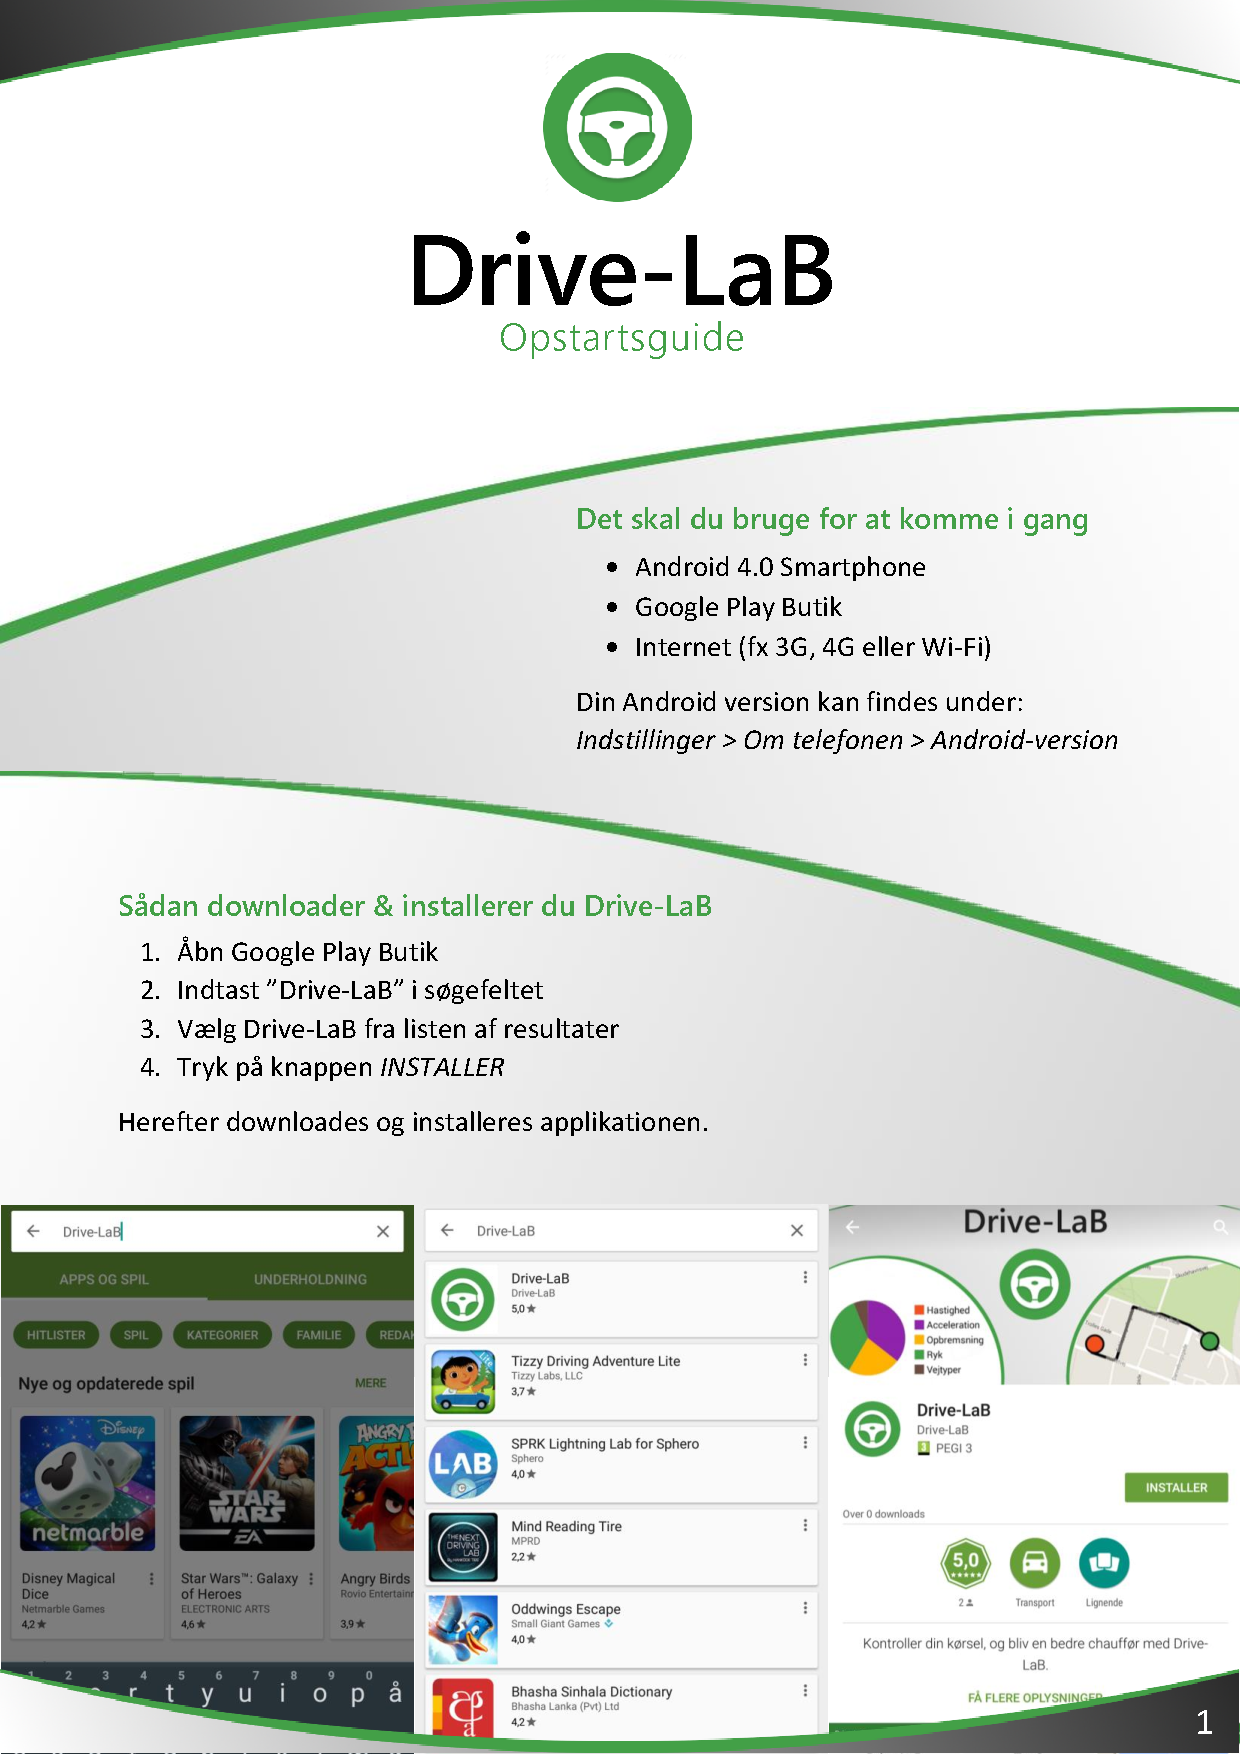
\includepdf[pages={1-}]{Appendix/Drive-LaB_Guide.pdf}
\subsection*{Data Warehouse}\label{app:datawarehouse}

\begin{figure}[tb]
\centering
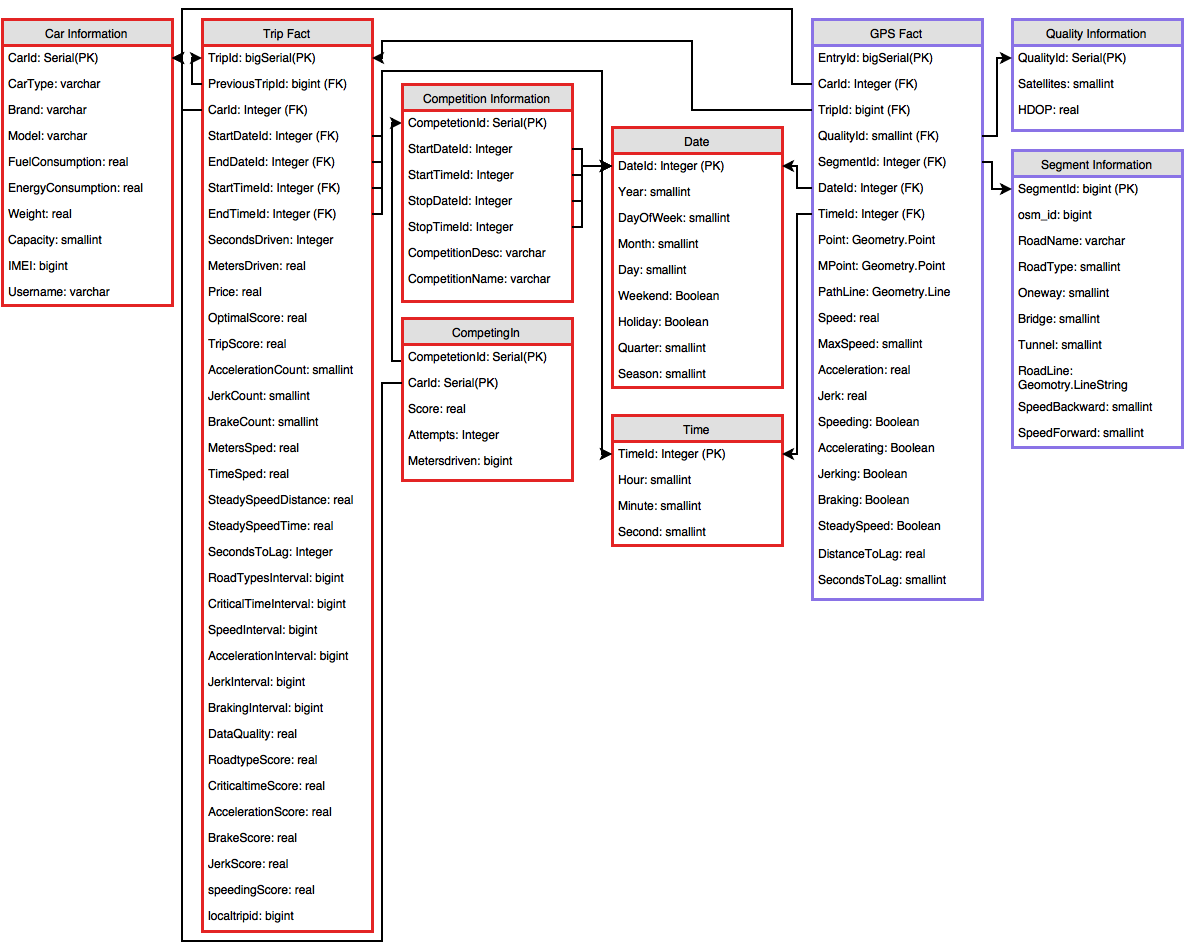
\includegraphics[width=0.95\textwidth]{Pictures/newdatawarehouse}
\caption{A picture of the entire data warehouse as it is used in the project}
\label{app:fig:newdatawarehouse}
\end{figure}

\end{document}